\chapter{Evaluation}
%
\section{GMT Characteristics}
%
\subsection{Characteristic Values of the Oscilloscope}
%
The signal of the GMT can be seen on the oscilloscope screen. \cref{subfig:fig1pulsAmplitude} shows the base line \(U_{0}\) and
the amplitude \(\hat{U}\):
%
\begin{align}
U_{0}   &=  \SI{24}{mV} \pm \SI{40}{mV} \\
\hat{U} &=  \SI{1,56}{V} \pm \SI{0,04}{V}
\end{align}
%
Further there can be read off the fall time \(t_{f}\) (\cref{subfig:fig2fallTime}), rise time \(t_{r}\) (\cref{subfig:fig3riseTime}), the pulse width \(t_{p}\)
(\cref{subfig:fig4pulseWidth}) and recovery time \(t_{r}\) (\cref{subfig:fig5recoveryTime}):
\begin{align}
t_{f}   &=  \SI{56}{\micro s} \pm \SI{20}{\micro s} \\
t_{r}   &=  \SI{228}{\micro s} \pm \SI{20}{\micro s} \\
t_{p}   &=  \SI{108}{\micro s} \pm \SI{20}{\micro s} \\
t_{re}  &=  \SI{288}{\micro s} \pm \SI{20}{\micro s}
\end{align}
%
\subsection{Characteristic Curve of the GMT}
%
After determining the starting voltage \(U_{start}\) to \(U_{start}=\SI{328}{V}\), the characteristic curve has been
recorded. The calculated mean value
of the count rate has been plotted versus the mean voltage by \textsc{SciDAVis}:\par
\begin{figure}[H]
 \centering
 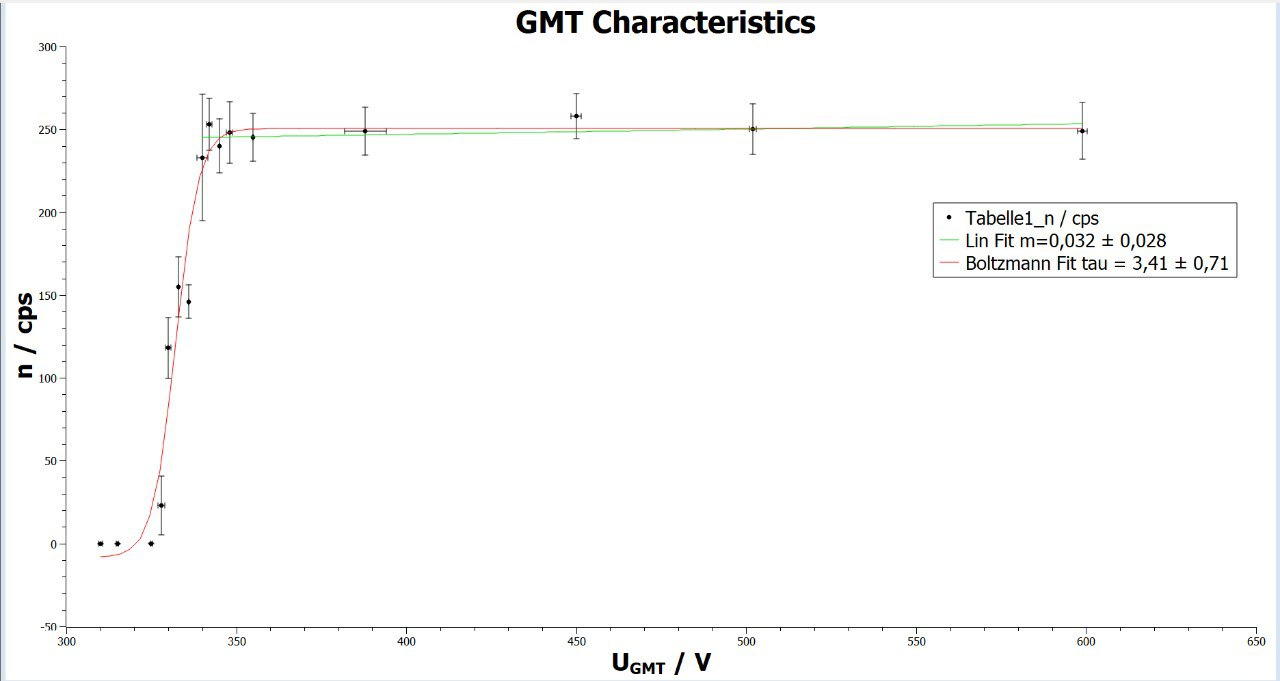
\includegraphics[width=.9\textwidth]{scidavis/Fig.6_GMT-characteristics.jpg}
 \caption[GMT characteristic]{Plot characterising the operating GMT.}
 \label{fig:gmtCharacteristics}
\end{figure}
The relative slope in the plateau area is determined to \(m=(3,2 \pm 2,8) \frac{\%}{\SI{100}{V}}\).\par
The optimum working voltage \(U_{opt}\) is determined to \(U_{opt}=\SI{500}{V}\), since the maximum possible adjustable
voltage of \(U_{GMT}=\SI{600}{V}\) is still in the plateau area, which starts at \(U_{GMT}=\SI{340}{V}\).
%
\section{Angular Dependency of the Count Rate}
To examine the angular dependency the count rate was measured at the optimum working voltage of
\(U_{opt}=\SI{500}{V}\) and the mean values of the 12 count rates of each angle were calculated. After that, the count
rate versus angle was given as:\par
\begin{figure}[H]
 \centering
 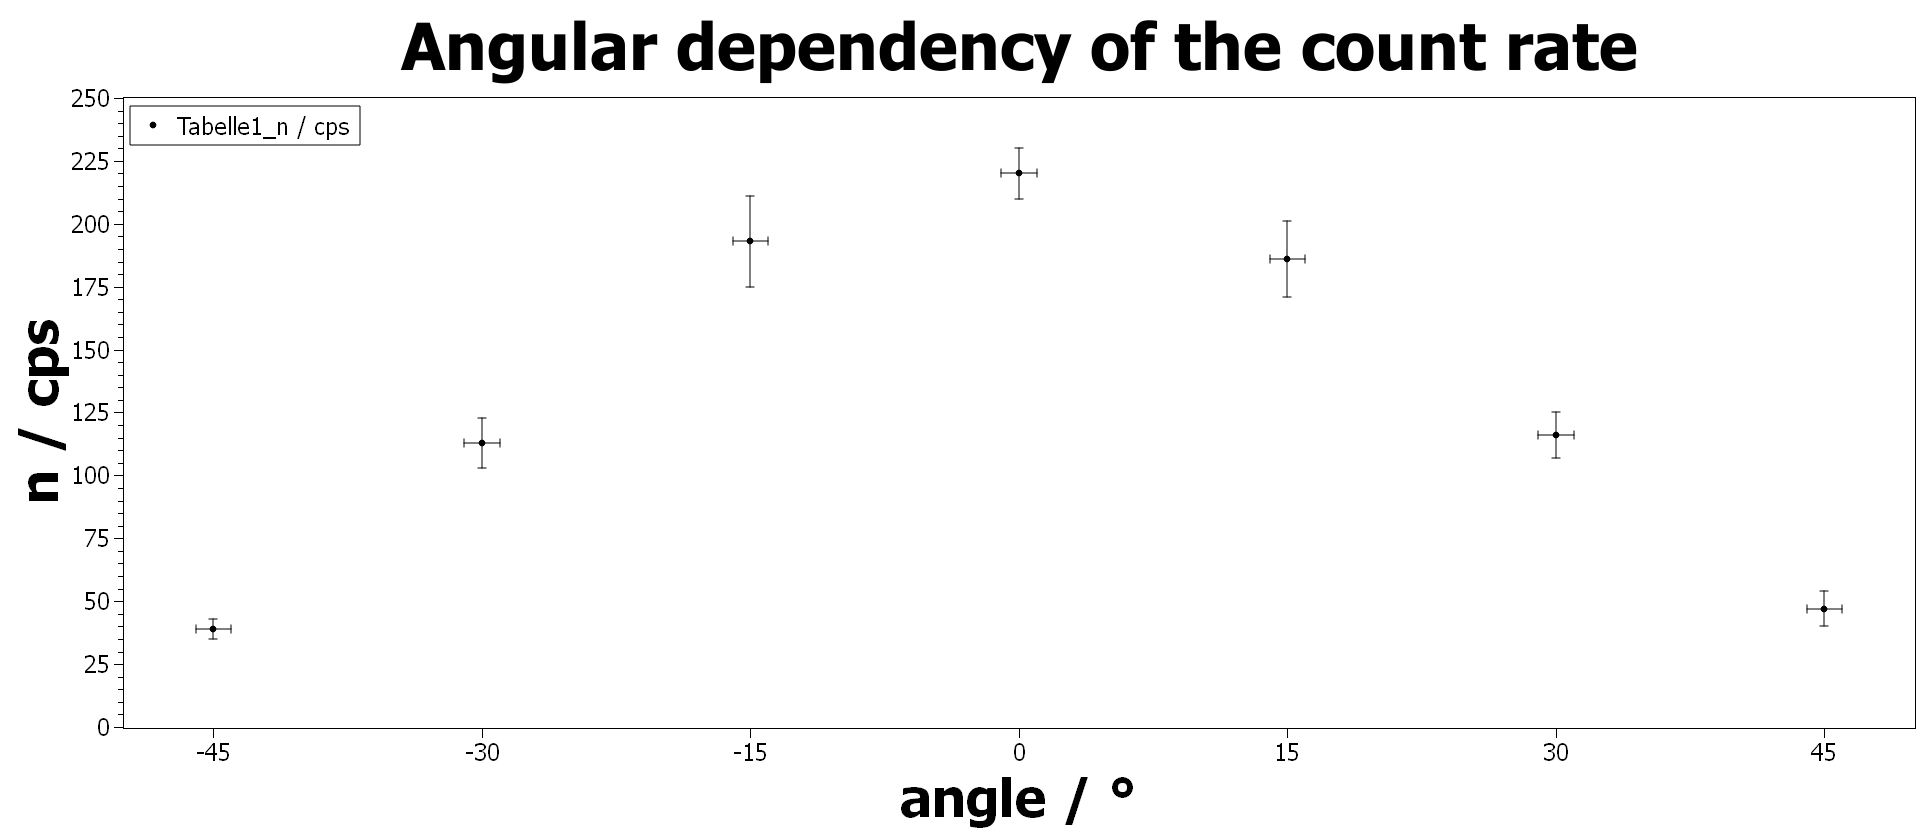
\includegraphics[width=.8\textwidth]{scidavis/Fig.7_Angular dependency of the count rate.jpg}
 \caption[Angular dependency of cps]{Angular dependency of the measured count rate.}
 \label{fig:angularDepCPS}
\end{figure}
%
\section{Absorption Characteristics of Materials}
%
For investigating the absorption characteristics of materials, the means of the count rates at
\(U_{opt}=\SI{500}{V}\) for different materials were determined:
%
\begin{align}
&\text{no absorbing material: }  &&n = \SI{221}{cps} \pm \SI{11}{cps}\\
&\text{Aluminum (Al): }          &&n = \SI{10}{cps} \pm \SI{4}{cps}\\
&\text{Lead (Pb): }              &&n = \SI{7}{cps} \pm \SI{2}{cps}\\
&\text{Tin (Sn): }               &&n = \SI{6}{cps} \pm \SI{2}{cps}\\
&\text{Acrylic glass: }          &&n = \SI{26}{cps} \pm \SI{5}{cps}\\
&\text{Cardboard: }              &&n = \SI{104}{cps} \pm \SI{8}{cps}
\end{align}
%
The explanation for the different absorption of the different materials is the mass attenuation coefficient of the
different materials. The mass attenuation coefficient is dependent on the material density and the attenuation
coefficient. Since the attenuation coefficient depends on the atomic number, the size of the atom does
matter. The reason why there is happening an attenuation is because of the \(\alpha\)-, \(\beta\)- and \(\gamma\)-rays are
interacting with the material atoms. While the \(\alpha\)- and \(\beta\)-rays have a strong interaction with the material,
\(\gamma\)-rays have better penetration due to less likeliness to interact. The smaller the half-value layer of a
material the weaker the penetration. With lead (\isotope[82]{Pb}) and Tin (\isotope[50]{Sn}) and presumably Aluminum
(\isotope[13]{Al}) as well almost all rays are absorbed (dependent on the ray energy). Acrylic glass can probably be
traversed by the \(\gamma\)-rays. Due to there size already a thin sheet of cardboard is sufficient to absorbed
\(\alpha\)-ray particles almost entirely.
%
\section{Counting Statistics}
%
After 90 measurements we obtained the following statistical values for mean \( \bar{n} \), variance \( \sigma^{2} \) and standard deviation
\( \sigma \):
%
\begin{align}
\bar{n}     &=  \SI{4327}{cps} \\
\sigma^{2}  &=  \SI{4168}{(cps)^{2}} \\
\sigma      &=  \SI{65}{cps}
\end{align}
The measurement series results in a scatter plot as shown in \cref{fig:countingStatistics}.
\begin{figure}[H]
 \centering
 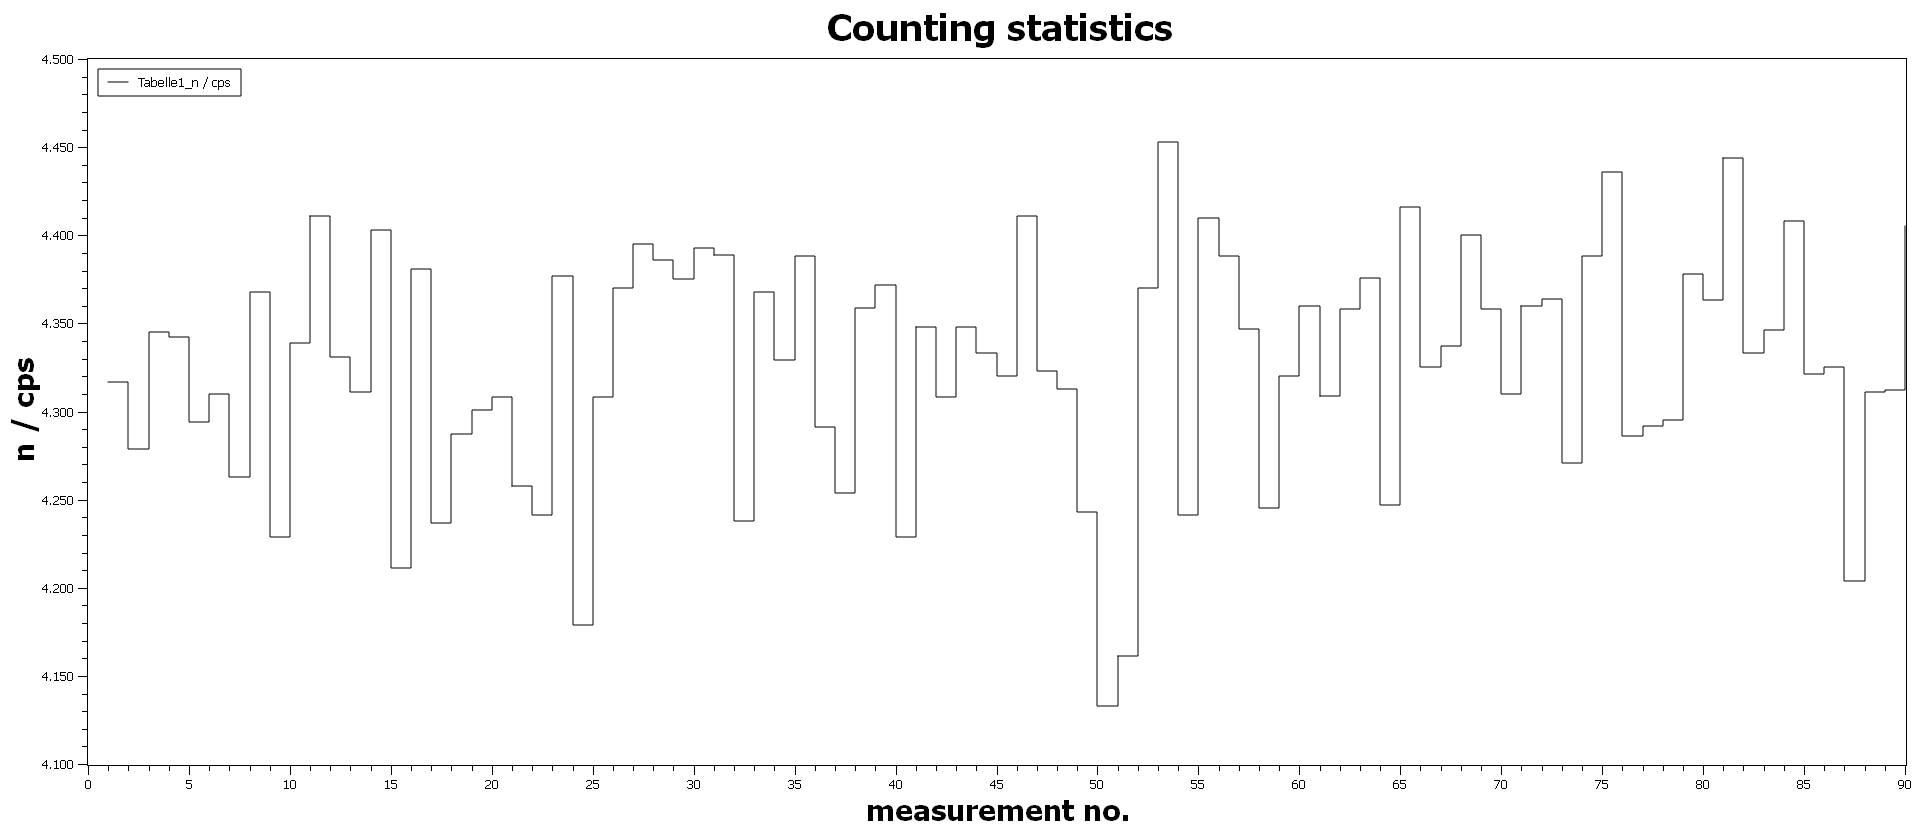
\includegraphics[width=.8\textwidth]{scidavis/Fig.8_Counting statistics.jpg}
 \caption[Counting statistics]{Counting statistics.}
 \label{fig:countingStatistics}
\end{figure}
with the associated histogram of distribution as seen in \cref{fig:countStatsHistogram}:
\begin{figure}[H]
 \centering
 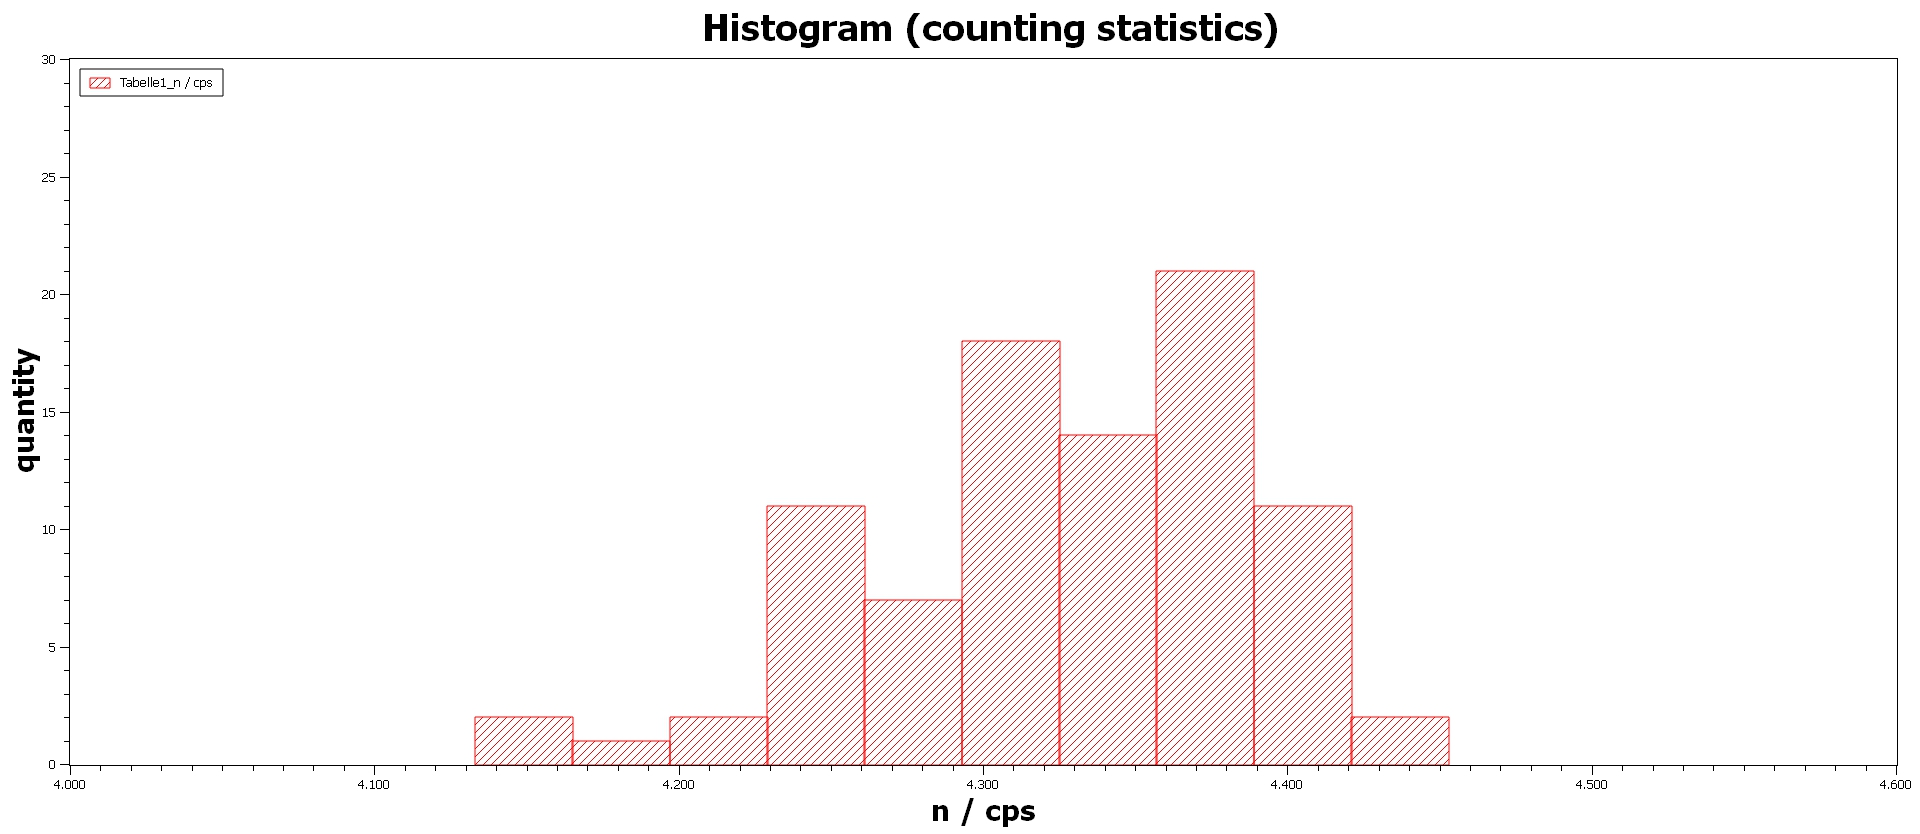
\includegraphics[width=.8\textwidth]{scidavis/Fig.9_Histogram (counting statistics).jpg}
 \caption[Histogram of the count rates]{Histogram of the count rates.}
 \label{fig:countStatsHistogram}
\end{figure}
With radioactive decay it cannot be said which atom will decay when. Since it is a statistical process, the histogram
can be described with a Poisson-distribution.
%
\section{Background Radiation}\label{sec:backgroundRadiation}
%
To investigate the background radiation the count rate was measured 90 times with no radiation source at a voltage of
\( U_{opt}=\SI{500}{V} \). The measurement stats are:
%
\begin{align}
\bar{n}     &=  \SI{3}{cps} \\
\sigma^{2}  &=  \SI{20}{(cps)^{2}} \\
\sigma      &=  \SI{4}{cps}
\end{align}
The measurement number was plotted versus the count rate:
\begin{figure}[H]
 \centering
 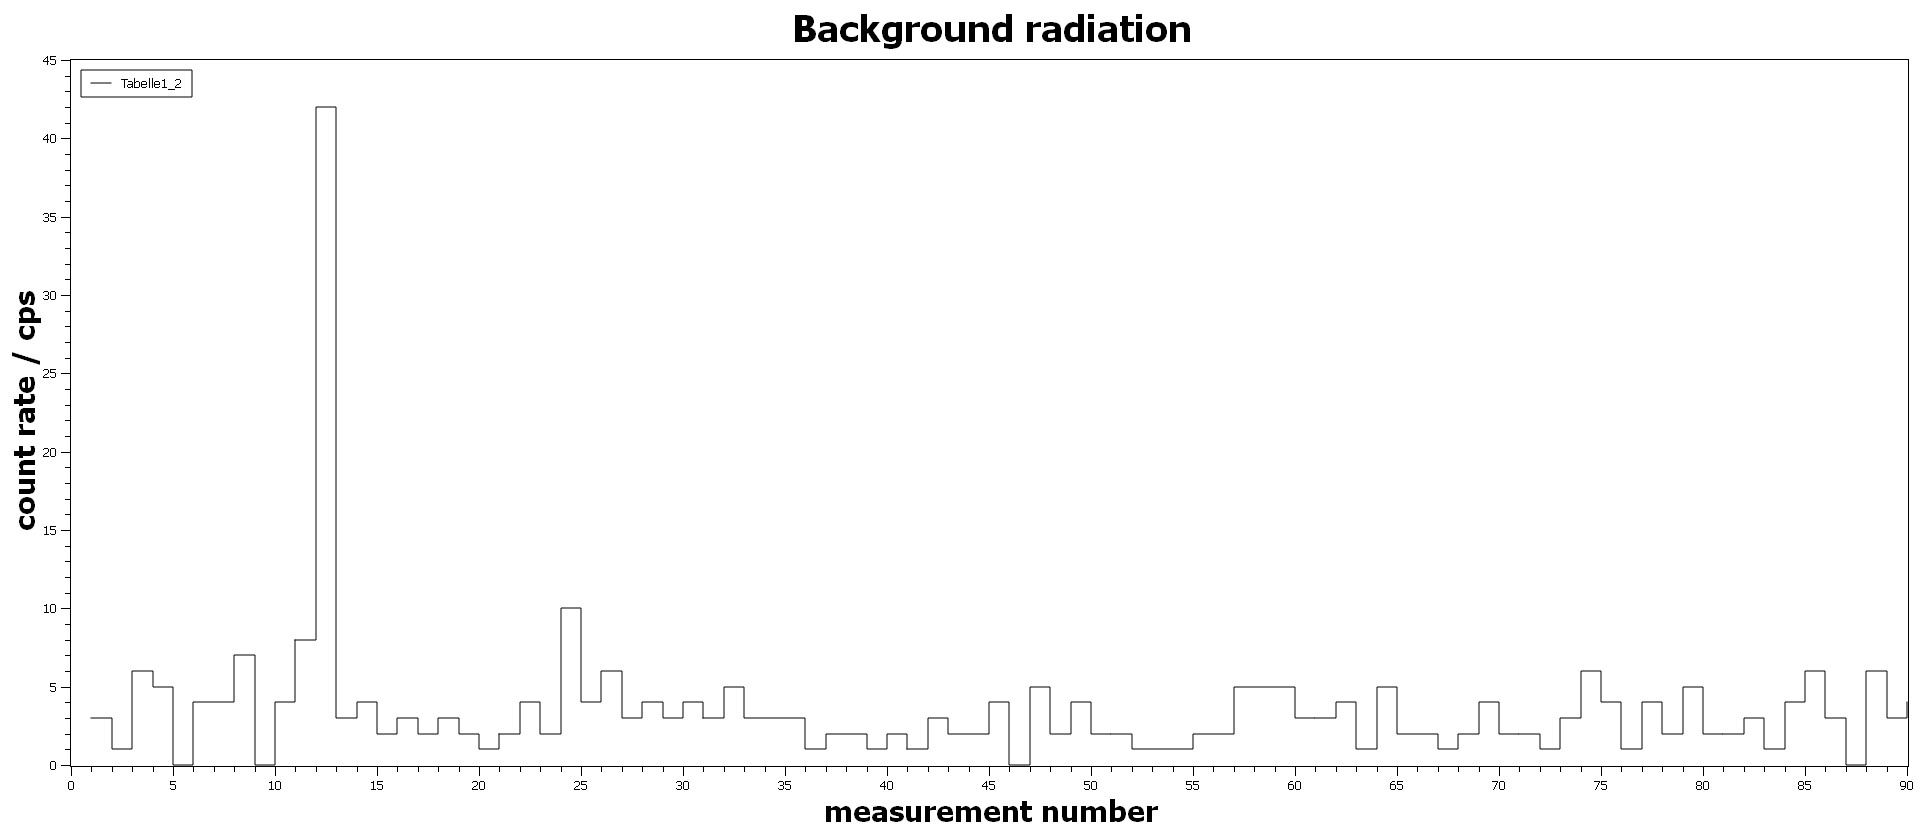
\includegraphics[width=.9\textwidth]{scidavis/Fig.10_Background radiation.jpg}
 \caption[Background radiation cps]{Measured counts caused by natural background radiation.}
 \label{fig:backgroundRad}
\end{figure}
With the associated distribution histogram:
\begin{figure}[H]
 \centering
 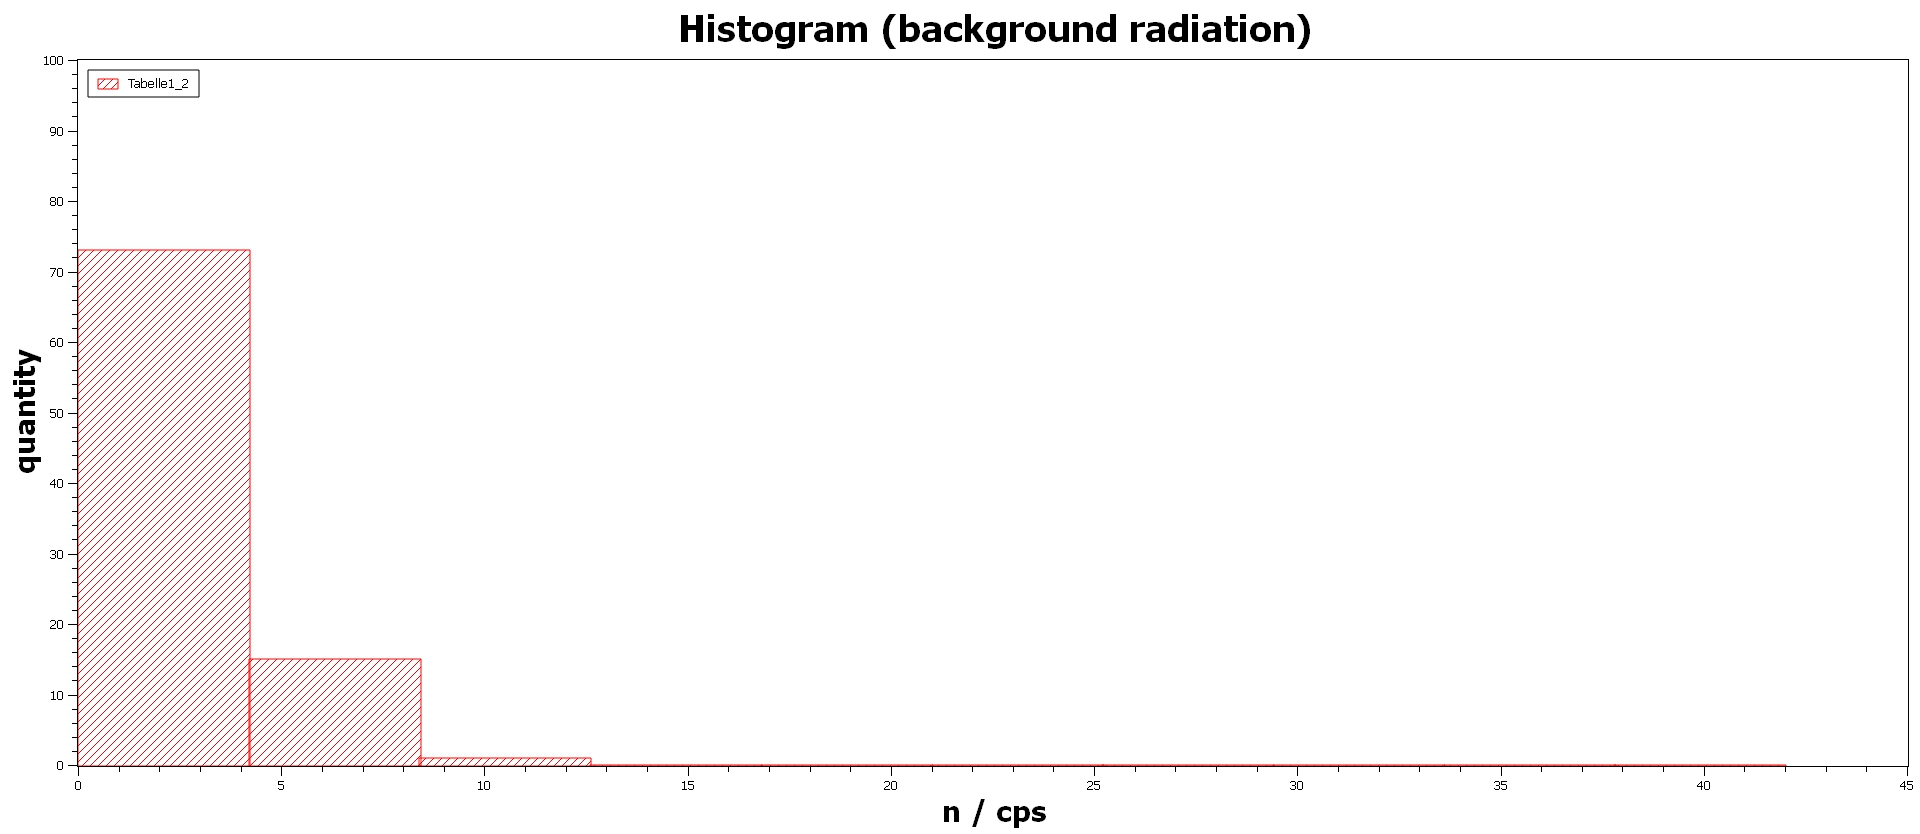
\includegraphics[width=.9\textwidth]{scidavis/Fig.11_Histogram (background radiation).jpg}
 \caption[Back Rad Hist]{Background Radiation Histogram.}
 \label{fig:backgroundRadHistogram}
\end{figure}
This histogram can also be described by a Poisson-distribution for the same reason as histogram of the counting
statistics.
%
\section{Natural Radioactivity}
%
Lastly, the radioactivity of Brazil Nuts was determined. The mean value of \( \bar{n}=\SI{3}{cps} \) indicates that the
radioactivity of the Brazil Nuts is very weak because it has the same mean value as the background radiation. However,
this does not have to mean that the Brazil Nuts do not emit any radiation. Because the tube was very close to the nuts,
the background radiation could not pass directly through the nuts, which implies that the rest of the radiation must have
come from the Brazil Nuts.
\begin{figure}[H]
 \centering
 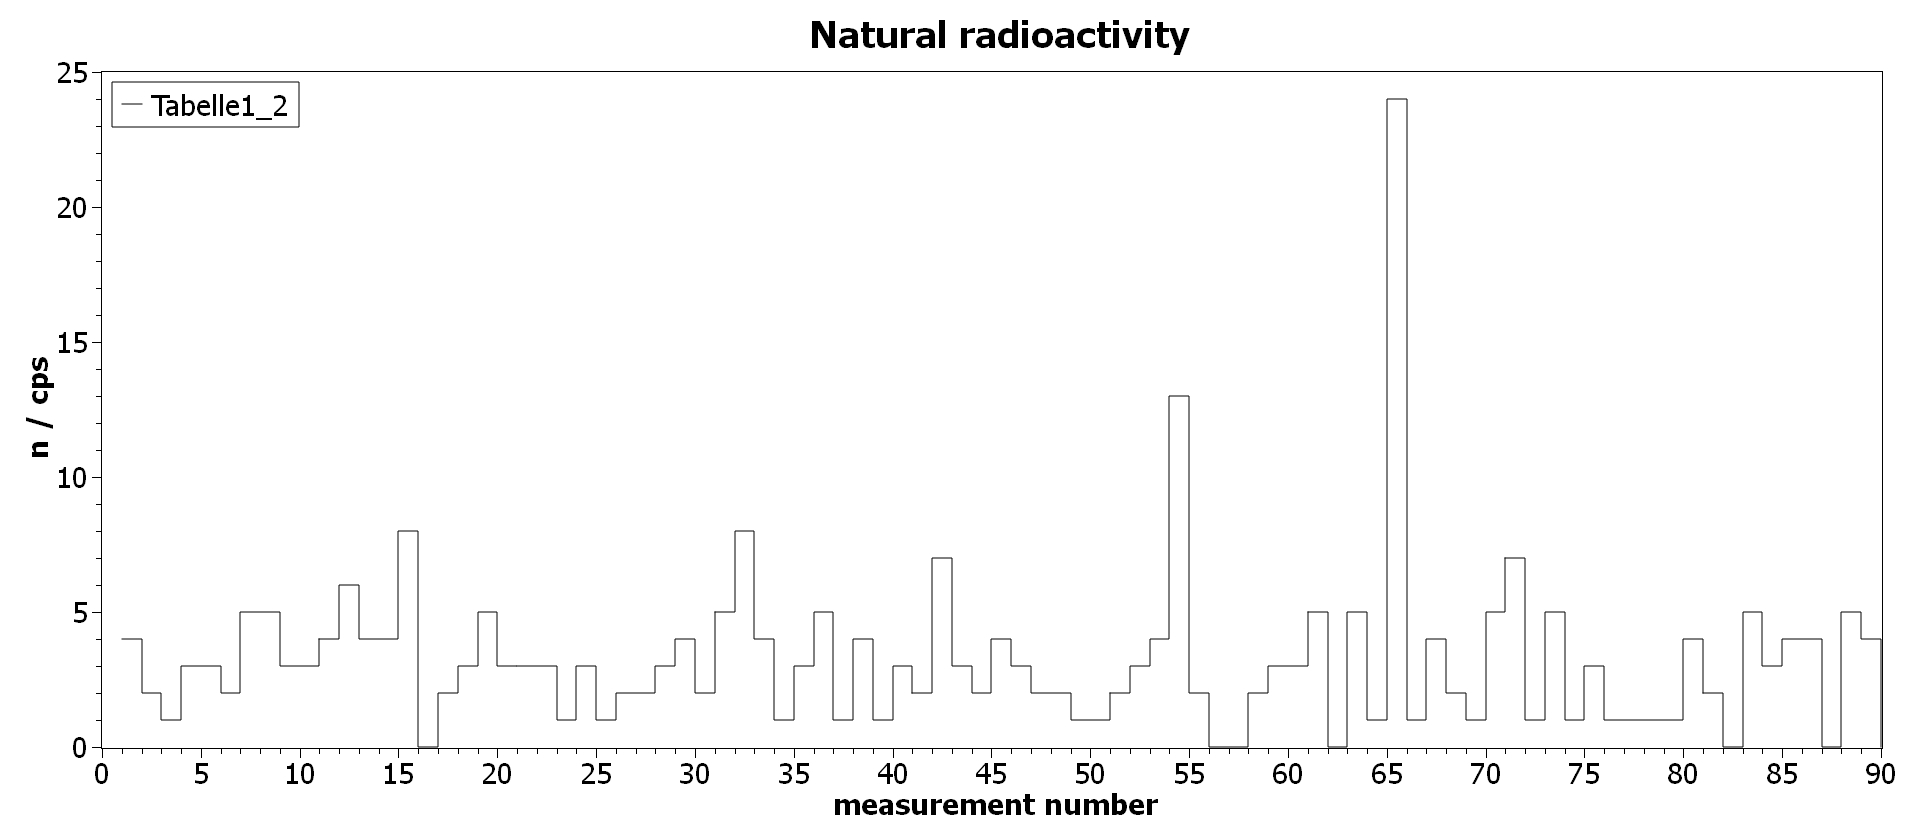
\includegraphics[width=.9\textwidth]{scidavis/Fig.12_Natural radioactivity.jpg}
 \caption[Brazil Nuts]{Radiation of Brazil Nuts.}
 \label{fig:brazilNutz}
\end{figure}